\documentclass[11pt,a4paper]{article}
\usepackage{{../../paquete}}
\usepackage{{../../estilos}}
\graphicspath{{../Figuras/}} %Esta es la forma en la que se insertan direcciones RELATIVAS ya que la carpeta Firugas y el documento se encuentran en la misma ubicación

%BEGIN_FOLD
\newcommand{\nombreMateria}{Máquinas Térmicas}
%END_FOLD.


\begin{document}
	\ProvidesPackage{portada}

\usepackage{tikz}
\usepackage{setspace}
\definecolor{maincolor}{HTML}{213250}

\makeatletter
\renewcommand{\maketitle}{
	\begin{titlepage}\centering
		\begin{tikzpicture}[remember picture, overlay]
			\draw[line width=60pt, color=maincolor] 
			([xshift=1cm, yshift=-1cm]current page.north west) 
			rectangle 
			([xshift=-1cm, yshift=1cm]current page.south east);
		\end{tikzpicture}
		\vfill
		
\includegraphics[width=4cm]{recursos/logo}\\[5pt]
		{\Large \textsc{Universidad Tecnológica Nacional}\\[5pt]
			Facultad Regional Reconquista\\[5pt]
			Ingeniería Electromecánica}\\[3cm]
		
		\begin{minipage}{.7\linewidth}
			\centering
			\setstretch{.9}
			{\Huge\textbf{\@title}\\[5pt]
				\LARGE \emph{Apunte de Cátedra} \par}
			\vspace{3cm}
		\end{minipage}
		\vfill
		{\@author\\[5pt]
			\large \@date}
		\vfill
	\end{titlepage}
}
\makeatother

	\pagestyle{fancy}
	%Includesss
		\section{Introducción general}

\vspace{-.5cm}

\subsection{Conceptos básicos}

\subsubsection{Energía} La energía es una característica de la materia y puede transformarse o transferirse. Existen en la naturaleza de distintas maneras.
Así por ejemplo denominamos energía hidráulica (potencial gravitatoria) a la obtenida de dos niveles de agua; energía eólica (cinética) a la energía obtenida por la acción de los vientos; energía química a la obtenida por combustionar un combustible industrial; y, energía nuclear a la liberada por fisión o fusión de los combustibles nucleares. Utilizando cualesquiera de ellas podemos obtener, a través de una máquina, energía eléctrica.

\subsubsection{Máquina} 

Técnicamente se denomina máquina a todo dispositivo capaz de transformar y/o transferir energía.



Las máquinas de fluidos utilizan \textsl{fluidos de trabajo} para generar energía y se clasifican en dos grandes grupos: \textsl{máquinas hidráulicas}, como las turbinas hidráulicas que transforman la energía cinética del agua en energía mecánica de rotación; y en \textsl{máquinas térmicas}, como las turbinas de vapor, donde el funcionamiento es similar a una turbina hidráulica exceptuando el cambio de propiedades que sufre el líquido de trabajo durante el transcurso.

\subsection{Clasificación de las máquinas de los fluidos}


\subsubsection{Máquinas Hidráulicas} Una máquina hidráulica utiliza como fluido de trabajo a los fluidos incompresibles o aquellos que se comporten como tal debido a que en el interior del sistema no sufren variaciones significativas en sus propiedades.
\subsubsection{Máquinas Térmicas} Es un dispositivo que transforma energía pero su fluido de trabajo cambia sus propiedades durante la operación de la máquina.

Se clasifican en dos: 
\begin{itemize}
	\item Turbomáquinas.
	\item De desplazamiento positivo.
\end{itemize}

En las \textsl{turbomáquinas} la sustancia de trabajo es impulsada a traves de un rotor provisto de palas y cuyo principio de funionamiento se basa en las ecuaciones de Euler. 	

\subsection{Aplicaciones de las Máquinas Térmicas}
\subsubsection{Turbinas de vapor}
\subsubsection{Turbinas de gas}
\subsubsection{Turbocompresores}
\subsubsection{Motoras}
\subsubsection{Generadoras}

\subsection{Ecuaciones de Euler}
\subsection{Principio de desplazamiento positivo}
\lipsum[2]
	\hyphenation{cal-de-ras}
\section{Combustibles para calderas}
\subsection{Combustibles}

\begin{preguntas}
	. ¿Qué es un combustible?
\end{preguntas}

Un combustible es cualquier sustancia que, por un proceso químico de oxidación exotérmica\footnote{La palabra ``exotérmica'' se refiere a una reacción que libera energía térmica hacia el entorno.} o por un proceso físico de fisión o fusión, suministra energía en forma de calor.\\

Aquellas sustancias que cumplen con el primer proceso, se las denomina \textbf{combustibles industriales}. Liberan energía en forma de calor sin generar gases nocivos para el ser humano.
Esta distinción es importante, considerando que existen materiales que al quemarse producen gases tóxicos y corrosivos, como el azufre.\\

Por otro lado, el combustible que cumple con el segundo proceso es denominado como \textbf{combustible nuclear}. La combustión de estas sustancias liberan partículas radiactivas perjudiciales para la salud, lo cual implica que su uso debe llevarse a cabo en condiciones estrictas de aislamiento.

\subsection{Combustión}

La combustión es una reacción química de oxidación exotérmica donde la \textsl{energía liberada} se da en forma de \textsl{calor}. El agente oxidante ocomburente en dicha reacción es el oxígeno del aire.\\

A altas temperaturas el combustible reacciona con el aire para generar luz y gases de combustión:

\begin{equation}
	\textsl{Combustible} + \textsl{Aire} \rightarrow \textsl{Radiación} + \textsl{Gases de combustión}
\end{equation}


El combustible puede ser sólido, líquido o gaseoso, y los gases de combustión transportarán la energía en forma de calor.\\

Al ser el proceso de combustión muy complejo y con vista en aplicaciones prácticas, el estudio que se realiza en la materia \materia\ considera factores estáticos, es decir, la determinación de los estados finales e iniciales del proceso de combustión. Los resultados obtenidos a través de esta simplificación son suficientes para resolver los problemas.

\subsubsection{Tipos de combustión}

A continuación se muestran los tipos de combustión que pueden tener lugar en la reacción química.

\begin{itemize}
	\item \textbf{Combustión completa:} tiene lugar cuando \textsl{todo} el combustible se quema en presencia de suficiente oxígeno.
	\item \textbf{Combustión perfecta:} ocurre en condiciones ideales, es decir, en un entorno \textsl{libre de impurezas} y con una cantidad ilimitada de oxígeno disponible.
	\item \textbf{Combustión incompleta:} ocurre cuando un combustible se quema en presencia de una cantidad insuficiente de oxígeno, es decir, no todos los átomos del combustible se combinan con oxígeno para formar dióxido de carbono y agua, por lo que \textsl{producen subproductos} adicionales, como monóxido de carbono, alquitrán y otros hidrocarburos.
	\item \textbf{Combustión imperfecta:} se refiere a una combustión incompleta que ocurre cuando un combustible se quema en presencia de una cantidad limitada de oxígeno.
\end{itemize}


La principal diferencia entre la combustión completa y perfecta es que la última se produce bajo condiciones ideales y no produce subproductos, mientras que la combustión completa simplemente implica que todo el combustible se quema en presencia de suficiente oxígeno, sin tener en cuenta las impurezas y otros factores que pueden afectar la reacción.


Y la principal diferencia entre la combustión incompleta e imperfecta es la cantidad de oxígeno presente en la reacción. Además, la combustión incompleta es más peligrosa que la combustión imperfecta debido a la mayor cantidad de subproductos tóxicos que produce.

\subsubsection{Cálculo de aire mínimo o teórico}

\subsection{Poder calorífico}
El poder calorífico es la cantidad de energía liberada como calor en un proceso de combustión.

Se debe utilizar aquel combustible con mayor poder calorífico, aunque en la práctica no ocurre debido a la disponibilidad del combustible y su costo. También, otra limitación es cuando se tiene en cuenta la contaminación que pudiera llegar a producir a causa del humo de combustión.
	

\subsubsection{Poder Calorífico Superior}

\subsubsection{Poder Calorífico Inferior}
<<<<<<< HEAD
	\hyphenation{cal-de-ras}
\section{Generadores de vapor}

\subsection{Generalidades}

	IRAM-IAP-N°25/5 - ``\textit{Generadores de vapor y calderas de agua caliente}'' define como \textit{generador de vapor} al conjunto constituido por la caldera de vapor con alguno o todos de los siguientes aparatos intercambiadores de calor:
	\begin{itemize}
		\item \textbf{Sobrecalentador:} se utiliza en las calderas para aumentar la temperatura del vapor generado por encima de su punto de saturación. Esto se logra al transferir calor adicional al vapor después de que ha sido generado en la caldera. El sobrecalentador ayuda a mejorar la eficiencia y el rendimiento del sistema al proporcionar vapor seco y sobrecalentado.
		
		\item \textbf{Desobrecalentador:} se utiliza para reducir la temperatura del vapor sobrecalentado. Su función principal es enfriar el vapor y asegurarse de que no exceda los límites de temperatura deseados antes de entrar en ciertos componentes o procesos posteriores.
		
		\item \textbf{Recalentador:} se utiliza para aumentar la temperatura del vapor. Sin embargo, a diferencia del sobrecalentador, coloca en una ubicación específica dentro del ciclo de vapor para volver a calentar el vapor después de que ha pasado por una etapa de expansión. Esto ayuda a aumentar la eficiencia térmica del sistema.
		
		\item \textbf{Economizador:} se utiliza para aprovechar el calor residual de los gases de escape de la caldera y transferirlo al agua de alimentación de la caldera. Al precalentar el agua de alimentación antes de entrar en la caldera, se logra un ahorro de energía al reducir la cantidad de calor requerido para generar vapor.
		
		\item \textbf{Calentador de aire:} se utiliza para calentar el aire que se suministra a un proceso o sistema. El aire frío que ingresa al calentador de aire se calienta al hacerlo pasar a través de tubos o conductos donde se transfiere calor desde una fuente de calor, como el vapor o los gases de escape. El aire caliente resultante se utiliza en diversas aplicaciones industriales o comerciales que requieren aire caliente.
	\end{itemize}

\subsection{Calderas}

La caldera, frente a los demás dispositivos, es el elemento principal e indispensable de un generador de vapor ya que los otros pueden no existir. La instalación o no de el resto de intercambiadores de vapor influirá en la calidad de vapor que se desee obtener y la conveniencia de aprovechar la energía calorífica que aún contienen los gases de combustión luego de su paso por la caldera.

\subsubsection{Clasificación}

En general, y a efectos de la materia \materia\ las calderas se clasifican según cómo circula el agua y el humo por las mismas. De esta manera, se distinguen dos tipos: calderas humotubulares o pirotubulares, y calderas acuotubulares.

\begin{figure}[!h]
	\centering
	\begin{subfigure}[b]{.4\linewidth}
		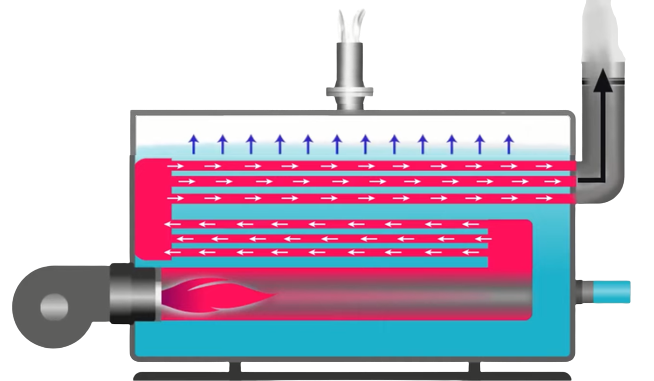
\includegraphics[width = \linewidth]{humotubular}
		\caption{Caldera humotubular}
		\label{fig:caldera-humo}
	\end{subfigure}
	\begin{subfigure}[b]{.4\linewidth}
		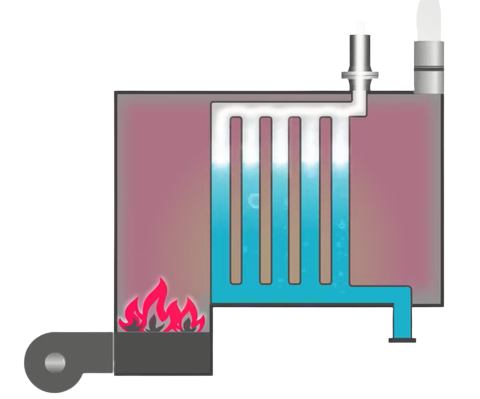
\includegraphics[width = \linewidth]{acuotubular}
		\caption{Caldera acuotubular}
		\label{fig:caldera-acuo}
	\end{subfigure}
	\caption{Tipos de calderas}
\end{figure}

\minisection{Calderas humotubulares}

Las calderas humotubulares (figura \ref{fig:caldera-humo}) son aquellas en la cual los gases de combustión o humos circulan por el interior de tubos que se encuentran sumergidos en el agua de la caldera (agua a vaporizar). Se definen en las normas como aquellas que cuentan con un ``cuerpo de la caldera'', el cual es una envolvente cilíndrica cerrada donde se produce la circulación del agua y se mantiene su nivel en el caso de calderas de vapor, o donde se produce el calentamiento del agua en el caso de calderas de agua caliente.

Dentro de este ``cuerpo'', se disponen haces de tubos con diámetros relativamente pequeños por los cuales circulan los gases de combustión o humos.


Este tipo de calderas ofrece una distribución más uniforme del calor en la masa de agua, lo que resulta en una generación de vapor y un rendimiento más uniforme en comparación con las calderas acuotubulares. Además, su puesta en marcha es más rápida. Su posición puede ser horizontal, con hogar exterior, o vertical, con hogar interior.



En la actualidad son más utilizadas las calderas humotubulares de hogar interior, quemando un combustible industrial líquido o gaseoso permitiendo una producción de vapor d ehasta $15\frac{tn}{h}$.


Las humotubulares verticales se utilizan para bajas producciones de vapor y presiones de hasta $15\frac{kg}{cm^2}$


\minisection{Calderas acuotubulares}

En las calderas acuotubulares (figura \ref{fig:caldera-acuo})

\subsubsection{Zonas de una caldera}

\minisection{Zona de liberación de calor}

En esta zona, llamado hogar, el calor se transfiere al agua principalmente por radiación. Es una zona crítica desde el punto de vista de resistencia de los materiales. 

\minisection{Zona de tubos}

Es la zona donde los gases, productos de la combustión, transfieren calor al agua principalmente por convección a medida que circulan por su circuito.

\subsubsection{Partes de una caldera}

\begin{enumerate}
	\item \textbf{Hogar} 
	
	El hogar es el espacio dentro de la caldera donde se realiza la combustión del combustible y la liberación de calor, generalmente ubicada en la parte inferior de la caldera. El mismo puede estar situado de dos formas:
	\begin{itemize}
		\item En el interior, donde se encuentra dentro de un recipiente metálico rodeado de paredes refrigeradas con agua.
		\item En el exterior, donde está construido fuera del recipiente metálico y puede estar parcialmente rodeado o sin paredes refrigeradas.
	\end{itemize}
	
	Se puede clasificar según el tipo de combustible, para sólidos o gaseosos; o el tipo constructivo, de tubo liso o corrugado.
	\item \textbf{Puerta de hogar}
	
	Es una pieza metálica robusta con abisagrada que puede tener varias funciones según el tipo de caldera. Si se trata de un combustible sólido, es utilizada para la \textit{carga manual del combustible} y la \textit{inspección de la llama}. Si se quema combustible líquido o gaseoso, esta puerta se reemplaza por un quemador.
	
	\item \textbf{Emparrillado}
	
	Es una estructura metálica de forma enrejada y sirve de apoyo para el combustible sólido depositado en el hogar. Permite el ingreso de aire primario para dr origen a la combustión.
	
	
	Según su diseño puede ser \textit{parrilla fija}, seca o húmeda; o \textit{parrilla móvil}, como transportadores, reciprocantes o basculantes.\\
	
	Un buen emparrillado debe cumplir con las siguientes condiciones:
	\begin{itemize}
		\item Permitir el paso del aire primario.
		\item Permitir que las cenizas caigan hacia el cenicero.
		\item Que se limpie con facilidad y rapidez.
		\item Impedir la acumulación de escoria.
		\item Ser construidos con materiales de buena calidad para que no se quemen, deformen y perduren en el tiempo.
	\end{itemize}

	\item \textbf{Cenicero}
	
	Es el espacio que queda bajo la parrilla y sirve para recoger las cenizas que caen. Los residuos acumulados deben ser retirados periódicamente para no obstaculizar el paso del aire primario.
	
	
	La extracción de las cenizas puede ser manual o mecanizada.
	
	\item \textbf{Puerta del cenicero}
	
	De igual características constructivas que la puerta del hogar, esta se utiliza para realizar funciones de limpieza del cenicero. Además, con esta puerta se puede regular la entrada de aire primario si la caldera no tiene tiraje forzado.
	
	\item \textbf{Altar}
	
	Es un pequeño muro de ladrillo refractario, debiendo pasar una altura aproximada de 30 cm, ubicado en el extremo opuesto a la puerta del fogón y al final de la parilla. Las funciones del altar son:
	\begin{itemize}
		\item Impedir que caigan a la parrilla partículas de combustible sin quemar.
		\item Ofrecer resistencia a la llama y gases para que estos se distribuyan a lo ancho del hogar pudiendo entregar la mayor parte de su energía al agua.
		\item En algunos casos sirve para ubicar boquillas para el ingreso de aire secundario.
	\end{itemize}

	\item \textbf{Mampostería}
	
	La mampostería es la construcción de ladrillos refractarios y comunes que tienen por objetivo \textit{cubrir la caldera} para minimizar las pérdidas de calor, y \textit{guiar los gases} y humos calientes en su recorrido.
	
	
	Para mejorar la aislación, a veces se construyen paredes con espacios huecos.
	
	
	En la actualidad, en algunos tipos de calderas se ha eliminado totalmente la mampostería de ladrillo, colocándose aislación térmica con materiales tales como lana de vidrio de alta densidad recubierta con chapas metálicas galvanizadas o inoxidables.
	
	\item \textbf{Conductos de humo}
	
	Son los espacios por los cuales circulan los humos y gases calientes de la combustión.
	
	\item \textbf{Caja de humo}
	
	Corresponde al espacio de la caldera en el cual se juntan los humos después de haber entregado su energía y antes de salir por la chimenea.
	
	\item \textbf{Chimenea}
	 
	Es un tubo que puede ser construido de mampostería o de chapa de acero. Se utiliza para conducir los gases de combustión a la atmósfera, ademas tiene la función de producir un tiraje natural.
	
	\item \textbf{Reguladores de tiro}
	
	Consiste en una compuerta metálica instalada en el conducto de humo que comunica con la chimenea o bien en la chimenea misma. Tiene por objetivo regular la cantidad de aire necesario para la combustión en función de la demanda de vapor, a su vez, ayuda a regular el paso de los gases de combustión a la salida.
	
	\item \textbf{Cilindro o tambor}
	
	El tambor de la caldera está diseñado para almacenar agua y vapor. En las calderas de tipo acuotubular, se encuentra conectado a una serie de tubos en los cuales circulan los gases calientes provenientes de la combustión. Estos tubos se encuentran sumergidos en el agua del tambor, lo que permite transferir el calor de los gases al agua y generar vapor.
	En el tambor se pueden diferenciar dos zonas principales: la cámara de agua y la cámara de vapor.
	
	La cámara de agua en el tambor de una caldera es un espacio específico dentro del tambor donde se ubica el nivel de agua y se lleva a cabo la separación entre el vapor y el agua líquida.
	
\end{enumerate}   

	
=======
	\section{Combustión para la generación de vapor}

\subsection{Definición de combustión}
La combustión es una reacción química que se produce entre el oxígeno y un material oxidable, que va acompañada de desprendimiento de energía y habitualmente se manifiesta por incandescencia o llama.

\subsection{Temperatura de ignición}


La temperatura de autoignición o de inflamación es la temperatura mínima a la que un combustible a presión atmosférica estándar, en presencia de oxígeno (aire), puede encenderse y quemarse sin necesitar una fuente externa de calor. Es importante mencionar que esta temperatura puede variar dependiendo del tipo de combustible, ya que diferentes sustancias tienen diferentes puntos de autoignición.

\subsection{Comburente y Combustible}

\subsubsection{Comburente}
Un \emph{comburente} es una sustancia que proporciona el oxígeno necesario para que ocurra la combustión. Actúa como el agente oxidante en una reacción de combustión al suministrar el oxígeno necesario para que los combustibles ardan.


Para cálculos estequiométrico en la materia de \materia consideramos al aire (aire técnico) compuesto por un 79\% de nitrógeno ($N$) y un 21\% de oxígeno ($O_2$)

\subsubsection{Combustible}
El \emph{combustible} es una sustancia que tiene la capacidad de arder o quemarse. Durante la combustión, el combustible reacciona con un comburente (como el oxígeno) liberando energía en forma de calor, luz u otros productos de reacción. Los combustibles pueden ser sólidos (como la madera o el carbón), líquidos (como la gasolina o el petróleo) o gaseosos (como el gas natural).



>>>>>>> cba4f4f0d8681eec39e6ae99405ad9a028227516
	
	
\end{document}